\documentclass{standalone}
\usepackage{tikz}
\usetikzlibrary{patterns, positioning}

\begin{document}
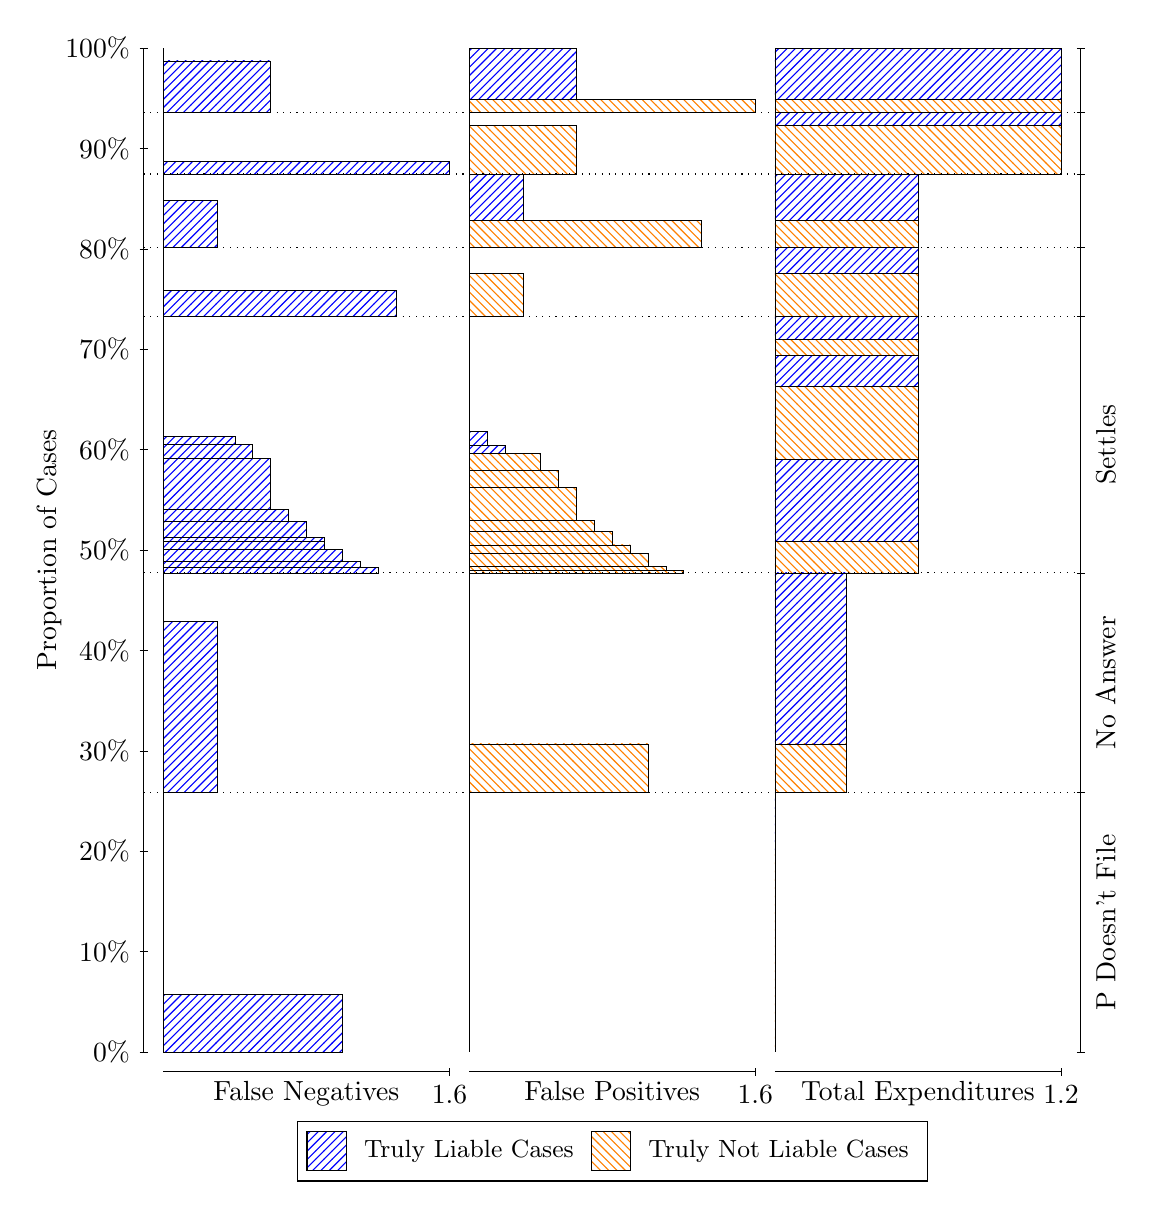
\begin{tikzpicture}
\draw[black, very thin] (1.5,1.75) -- (1.5,14.5);
\node[rotate=90, anchor=center] at (0.3, 8.125) {Proportion of Cases};
\draw[black, very thin] (1.45,1.75) -- (1.55,1.75);
\node[anchor=east] at (1.45, 1.75) {0\%};
\draw[black, very thin] (1.45,3.025) -- (1.55,3.025);
\node[anchor=east] at (1.45, 3.025) {10\%};
\draw[black, very thin] (1.45,4.3) -- (1.55,4.3);
\node[anchor=east] at (1.45, 4.3) {20\%};
\draw[black, very thin] (1.45,5.575) -- (1.55,5.575);
\node[anchor=east] at (1.45, 5.575) {30\%};
\draw[black, very thin] (1.45,6.85) -- (1.55,6.85);
\node[anchor=east] at (1.45, 6.85) {40\%};
\draw[black, very thin] (1.45,8.125) -- (1.55,8.125);
\node[anchor=east] at (1.45, 8.125) {50\%};
\draw[black, very thin] (1.45,9.4) -- (1.55,9.4);
\node[anchor=east] at (1.45, 9.4) {60\%};
\draw[black, very thin] (1.45,10.675) -- (1.55,10.675);
\node[anchor=east] at (1.45, 10.675) {70\%};
\draw[black, very thin] (1.45,11.95) -- (1.55,11.95);
\node[anchor=east] at (1.45, 11.95) {80\%};
\draw[black, very thin] (1.45,13.225) -- (1.55,13.225);
\node[anchor=east] at (1.45, 13.225) {90\%};
\draw[black, very thin] (1.45,14.5) -- (1.55,14.5);
\node[anchor=east] at (1.45, 14.5) {100\%};

\draw[black, very thin] (13.4,1.75) -- (13.4,14.5);
\draw[black, very thin] (13.35,1.75) -- (13.45,1.75);
\node[anchor=west] at (13.35, 1.75) {};
\draw[black, very thin] (13.35,5.0433) -- (13.45,5.0433);
\node[anchor=west] at (13.35, 5.0433) {};
\draw[black, very thin] (13.35,7.8351) -- (13.45,7.8351);
\node[anchor=west] at (13.35, 7.8351) {};
\draw[black, very thin] (13.35,11.089) -- (13.45,11.089);
\node[anchor=west] at (13.35, 11.089) {};
\draw[black, very thin] (13.35,11.971) -- (13.45,11.971);
\node[anchor=west] at (13.35, 11.971) {};
\draw[black, very thin] (13.35,12.9) -- (13.45,12.9);
\node[anchor=west] at (13.35, 12.9) {};
\draw[black, very thin] (13.35,13.685) -- (13.45,13.685);
\node[anchor=west] at (13.35, 13.685) {};
\draw[black, very thin] (13.35,14.5) -- (13.45,14.5);
\node[anchor=west] at (13.35, 14.5) {};

\draw[black, very thin, pattern color=blue, pattern=north east lines] (1.75,1.75) rectangle (4.0208,2.4802);
\draw[black, very thin, pattern color=orange, pattern=north west lines] (1.75,2.4802) rectangle (1.75,5.0433);
\draw[black, very thin, pattern color=blue, pattern=north east lines] (1.75,5.0433) rectangle (2.4312,7.2159);
\draw[black, very thin, pattern color=orange, pattern=north west lines] (1.75,7.2159) rectangle (1.75,7.8351);
\draw[black, very thin, pattern color=blue, pattern=north east lines] (1.75,7.8351) rectangle (4.475,7.9056);
\draw[black, very thin, pattern color=blue, pattern=north east lines] (1.75,7.9056) rectangle (4.2479,7.9817);
\draw[black, very thin, pattern color=blue, pattern=north east lines] (1.75,7.9817) rectangle (4.0208,8.1311);
\draw[black, very thin, pattern color=blue, pattern=north east lines] (1.75,8.1311) rectangle (3.7937,8.2365);
\draw[black, very thin, pattern color=blue, pattern=north east lines] (1.75,8.2365) rectangle (3.7937,8.2852);
\draw[black, very thin, pattern color=blue, pattern=north east lines] (1.75,8.2852) rectangle (3.5667,8.4927);
\draw[black, very thin, pattern color=blue, pattern=north east lines] (1.75,8.4927) rectangle (3.3396,8.6379);
\draw[black, very thin, pattern color=blue, pattern=north east lines] (1.75,8.6379) rectangle (3.1125,9.289);
\draw[black, very thin, pattern color=blue, pattern=north east lines] (1.75,9.289) rectangle (2.8854,9.4707);
\draw[black, very thin, pattern color=blue, pattern=north east lines] (1.75,9.4707) rectangle (2.6583,9.5701);
\draw[black, very thin, pattern color=orange, pattern=north west lines] (1.75,9.5701) rectangle (1.75,11.089);
\draw[black, very thin, pattern color=blue, pattern=north east lines] (1.75,11.089) rectangle (4.7021,11.419);
\draw[black, very thin, pattern color=orange, pattern=north west lines] (1.75,11.419) rectangle (1.75,11.971);
\draw[black, very thin, pattern color=blue, pattern=north east lines] (1.75,11.971) rectangle (2.4312,12.563);
\draw[black, very thin, pattern color=orange, pattern=north west lines] (1.75,12.563) rectangle (1.75,12.9);
\draw[black, very thin, pattern color=blue, pattern=north east lines] (1.75,12.9) rectangle (5.3833,13.062);
\draw[black, very thin, pattern color=orange, pattern=north west lines] (1.75,13.062) rectangle (1.75,13.685);
\draw[black, very thin, pattern color=blue, pattern=north east lines] (1.75,13.685) rectangle (3.1125,14.337);
\draw[black, very thin, pattern color=orange, pattern=north west lines] (1.75,14.337) rectangle (1.75,14.5);
\draw[black, very thin, pattern color=orange, pattern=north west lines] (5.6333,1.75) rectangle (5.6333,4.3131);
\draw[black, very thin, pattern color=blue, pattern=north east lines] (5.6333,4.3131) rectangle (5.6333,5.0433);
\draw[black, very thin, pattern color=orange, pattern=north west lines] (5.6333,5.0433) rectangle (7.9042,5.6624);
\draw[black, very thin, pattern color=blue, pattern=north east lines] (5.6333,5.6624) rectangle (5.6333,7.8351);
\draw[black, very thin, pattern color=orange, pattern=north west lines] (5.6333,7.8351) rectangle (8.3583,7.8639);
\draw[black, very thin, pattern color=orange, pattern=north west lines] (5.6333,7.8639) rectangle (8.1313,7.9157);
\draw[black, very thin, pattern color=orange, pattern=north west lines] (5.6333,7.9157) rectangle (7.9042,8.085);
\draw[black, very thin, pattern color=orange, pattern=north west lines] (5.6333,8.085) rectangle (7.6771,8.1903);
\draw[black, very thin, pattern color=orange, pattern=north west lines] (5.6333,8.1903) rectangle (7.45,8.3663);
\draw[black, very thin, pattern color=orange, pattern=north west lines] (5.6333,8.3663) rectangle (7.2229,8.5014);
\draw[black, very thin, pattern color=orange, pattern=north west lines] (5.6333,8.5014) rectangle (6.9958,8.9236);
\draw[black, very thin, pattern color=orange, pattern=north west lines] (5.6333,8.9236) rectangle (6.7687,9.1352);
\draw[black, very thin, pattern color=orange, pattern=north west lines] (5.6333,9.1352) rectangle (6.5417,9.3542);
\draw[black, very thin, pattern color=blue, pattern=north east lines] (5.6333,9.3542) rectangle (6.0875,9.4537);
\draw[black, very thin, pattern color=blue, pattern=north east lines] (5.6333,9.4537) rectangle (5.8604,9.6354);
\draw[black, very thin, pattern color=blue, pattern=north east lines] (5.6333,9.6354) rectangle (5.6333,11.089);
\draw[black, very thin, pattern color=orange, pattern=north west lines] (5.6333,11.089) rectangle (6.3146,11.641);
\draw[black, very thin, pattern color=blue, pattern=north east lines] (5.6333,11.641) rectangle (5.6333,11.971);
\draw[black, very thin, pattern color=orange, pattern=north west lines] (5.6333,11.971) rectangle (8.5854,12.307);
\draw[black, very thin, pattern color=blue, pattern=north east lines] (5.6333,12.307) rectangle (6.3146,12.9);
\draw[black, very thin, pattern color=orange, pattern=north west lines] (5.6333,12.9) rectangle (6.9958,13.522);
\draw[black, very thin, pattern color=blue, pattern=north east lines] (5.6333,13.522) rectangle (5.6333,13.685);
\draw[black, very thin, pattern color=orange, pattern=north west lines] (5.6333,13.685) rectangle (9.2667,13.848);
\draw[black, very thin, pattern color=blue, pattern=north east lines] (5.6333,13.848) rectangle (6.9958,14.5);
\draw[black, very thin, pattern color=orange, pattern=north west lines] (9.5167,1.75) rectangle (9.5167,4.3131);
\draw[black, very thin, pattern color=blue, pattern=north east lines] (9.5167,4.3131) rectangle (9.5167,5.0433);
\draw[black, very thin, pattern color=orange, pattern=north west lines] (9.5167,5.0433) rectangle (10.425,5.6624);
\draw[black, very thin, pattern color=blue, pattern=north east lines] (9.5167,5.6624) rectangle (10.425,7.8351);
\draw[black, very thin, pattern color=orange, pattern=north west lines] (9.5167,7.8351) rectangle (11.333,8.2322);
\draw[black, very thin, pattern color=blue, pattern=north east lines] (9.5167,8.2322) rectangle (11.333,9.2726);
\draw[black, very thin, pattern color=orange, pattern=north west lines] (9.5167,9.2726) rectangle (11.333,10.198);
\draw[black, very thin, pattern color=blue, pattern=north east lines] (9.5167,10.198) rectangle (11.333,10.599);
\draw[black, very thin, pattern color=orange, pattern=north west lines] (9.5167,10.599) rectangle (11.333,10.796);
\draw[black, very thin, pattern color=blue, pattern=north east lines] (9.5167,10.796) rectangle (11.333,11.089);
\draw[black, very thin, pattern color=orange, pattern=north west lines] (9.5167,11.089) rectangle (11.333,11.641);
\draw[black, very thin, pattern color=blue, pattern=north east lines] (9.5167,11.641) rectangle (11.333,11.971);
\draw[black, very thin, pattern color=orange, pattern=north west lines] (9.5167,11.971) rectangle (11.333,12.307);
\draw[black, very thin, pattern color=blue, pattern=north east lines] (9.5167,12.307) rectangle (11.333,12.9);
\draw[black, very thin, pattern color=orange, pattern=north west lines] (9.5167,12.9) rectangle (13.15,13.522);
\draw[black, very thin, pattern color=blue, pattern=north east lines] (9.5167,13.522) rectangle (13.15,13.685);
\draw[black, very thin, pattern color=orange, pattern=north west lines] (9.5167,13.685) rectangle (13.15,13.848);
\draw[black, very thin, pattern color=blue, pattern=north east lines] (9.5167,13.848) rectangle (13.15,14.5);
\draw[black, dotted] (1.5,5.0433) -- (13.4,5.0433);
\draw[black, dotted] (1.5,7.8351) -- (13.4,7.8351);
\draw[black, dotted] (1.5,11.089) -- (13.4,11.089);
\draw[black, dotted] (1.5,11.971) -- (13.4,11.971);
\draw[black, dotted] (1.5,12.9) -- (13.4,12.9);
\draw[black, dotted] (1.5,13.685) -- (13.4,13.685);
\draw[black, very thin] (1.75,1.5) -- (5.3833,1.5);
\node[anchor=north] at (3.5667, 1.5) {False Negatives};
\draw[black, very thin] (5.3833,1.45) -- (5.3833,1.55);
\node[anchor=north] at (5.3833, 1.45) {1.6};

\draw[black, very thin] (5.6333,1.5) -- (9.2667,1.5);
\node[anchor=north] at (7.45, 1.5) {False Positives};
\draw[black, very thin] (9.2667,1.45) -- (9.2667,1.55);
\node[anchor=north] at (9.2667, 1.45) {1.6};

\draw[black, very thin] (9.5167,1.5) -- (13.15,1.5);
\node[anchor=north] at (11.333, 1.5) {Total Expenditures};
\draw[black, very thin] (13.15,1.45) -- (13.15,1.55);
\node[anchor=north] at (13.15, 1.45) {1.2};

\node[black, centered, rotate=90] at (13.72, 3.3966) {P Doesn't File};
\node[black, centered, rotate=90] at (13.72, 6.4392) {No Answer};
\node[black, centered, rotate=90] at (13.72, 9.4622) {Settles};





\draw (7.449999999999999,1.5) node[draw=none] (baseCoordinate) {};
\begin{scope}[align=center]
        \matrix[scale=0.5, draw=black, below=0.5cm of baseCoordinate, nodes={draw}, column sep=0.1cm]{
            \node[rectangle, draw, minimum width=0.5cm, minimum height=0.5cm, pattern=north east lines, pattern color=blue] {}; &
            \node[draw=none, font=\small] (B) {Truly Liable Cases}; &
            \node[rectangle, draw, minimum width=0.5cm, minimum height=0.5cm, pattern=north west lines, pattern color=orange] {}; &
            \node[draw=none, font=\small] (B) {Truly Not Liable Cases}; \\
            };
\end{scope}

\end{tikzpicture}
\end{document}